% !TEX root = ../thesis.tex
% !TeX spellcheck = en_US

\section{Motivation}
	
	% finding good routes is difficult, solved using A*/Dijkstra on networks
	Traveling through a network of roads and paths often requires the use of a computer system determining the optimal route from a source to a destination location.
	The software used to solve this problem is often called a \emph{routing engine} and uses shortest path algorithms.
	A graph is used as the central data structure to abstract the real world into vertices and edges, which are points connected by lines representing roads and ways.
	Such graphs can represent non-physical networks as well, for example trading relationships between countries, social media networks or routers in the internet.
	However, only graphs representing road networks are considered in this thesis.
	
	Graphs can only model an abstraction of the real world.
	Detailed information regarding the geometry and infrastructure, such as the width or number of lanes, are usually added via attributes (usually key-value pairs) describing these properties.
	
	Algorithms for network-based routing, like the popular Dijkstra and A* algorithms, are well understood, optimized and used in numerous scientific and real-world applications.
	Over the last decades, optimizations and the use of more efficient data structures lead to further performance enhancements, making it possible to use such routing algorithms on large scale networks.
	% TODO I think this whole performance part can be removed
	Even though the performance is good enough for larger networks like the road network of the USA\cite{aviram-optimizing-dijkstra}, answering routing queries using normal shortest path algorithms on dense networks or networks of global scale are still a problem.
	To solve this, several speedup methods exist that further decrease query times, which will be covered later in \Cref{subsec:speedup-methods}.
	Using such techniques enables global routing request to be processed within milliseconds.\footnote{Tested for a routing request from Hamburg, Germany to Beijing, China on \href{https://www.openstreetmap.org/directions?engine=fossgis\_osrm\_car&route=53.55\%2C10.00\%3B39.91\%2C116.39}{openstreetmap.org} using the OSRM car profile which is based on Contraction Hierarchies (s. \Cref{subsubsec:ch}). The HTTP request returned the result in under 215ms -- including network latency of several milliseconds.}
	
	Aside from line-based shapes, which are very suitable for routing, the real world also consists of polygonal shapes like market places, parking lots or parks.
	Classical routing algorithms can only interpret the outer edges of these polygons as closed lines and therefore only find paths along these outer edges.
	Often, auxiliary paths are added to connect opposite sides of polygons, enabling routing algorithms to cross these areas.
	This is a common practice in OpenStreetMap, a crowdsourced geospatial database, for example on markets or playgrounds.
	Lower amounts of lines can be added quite easily by hand, but manually filling large areas or even a whole city with these auxiliary paths is not feasible.
	Fortunately, there are algorithms filling open spaces with edges as well as algorithms finding paths through open spaces without any additional edges.
	Both strategies will be covered in detail in following chapters.
	
	% problem: Most real world destinations are not on the network
	A similar problem arises with the source and destination locations of real-world routing.
	Because things like addresses, \term*{points of interest} (POIs) and manually chosen locations are often not part of roads or ways, they are rarely part of the underlying routing graph and therefore not reachable by classical routing algorithms.
	Even though there are algorithmic approaches to connect points to a graph (e.g. by searching for the nearest vertex on an edge), these simple approaches are often inaccurate.
	Such inaccuracies exist due to the space between an arbitrary location and the actual road network, which can contain numerous obstacles, such as walls or buildings.
	Furthermore, a walkable or drivable connection might not even exist at all, for example if the routing destination is located inside a lake.
	
	A third aspect is the quality of routes, which is limited when using classical routing algorithms due to the abstractions of the road network.
	Missing sidewalks, inaccurate geometries and missing connections between parallel ways put limits on the usefulness of graph-based routes, especially for routes determined for pedestrians.
	
	\begin{figure}[h]
		\begin{figcenter}
			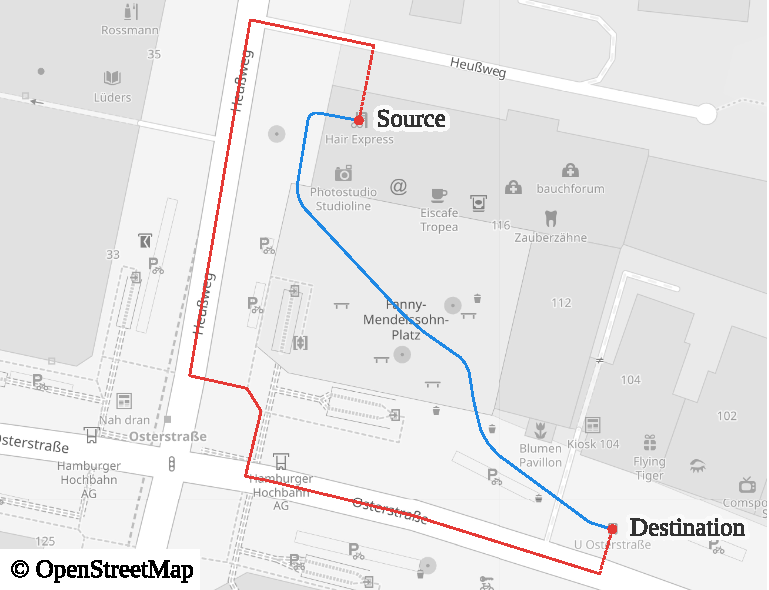
\includegraphics[width=0.5\textwidth]{images/qgis-routing-osterstrasse_expected-routing}
		\end{figcenter}
		\caption{A short route between two locations with the actually calculated route using a normal routing algorithm (red) and the shorter expected route a human would likely take (blue).}
	\end{figure}
	
	% alternative: geometric routing avoiding obstacles
	Besides graph-based routing algorithms, pure geometric routing approaches exist to determine shortest paths among obstacles in open spaces.
	Obstacles are geometries that cannot be passed under normal circumstances, like for example buildings, fences, lakes and walls.
	There are two main strategies to solve this type of shortest path problem\cite{hershberger-suri}:
	
	The first approach generates an auxiliary network around these obstacles (just like the aforementioned auxiliary paths) and then uses a graph-based shortest path algorithm to find the actual path.
	A variety of different approaches exist to generate such auxiliary edges\cite{graser-osm-open-spaces} which will be covered in detail in \Cref{subsec:visibility-graph}.
	
	The second approach does not create such a graph but stores its shortest path information for each source vertex in a map.
	This map consists of regions of equal predecessors, which means for a location in a specific region, the shortest path goes from the source vertex, via this predecessor vertex to the destination location this region.
	Details on geometric routing approaches are given in \Cref{subsec:continuous-dijkstra}.
	
\section{Problem and contributions}

	The previous section mentions one of the disadvantages of network-based routing:
	No assumptions can be made on whether source and destination locations are represented as vertices in the graph.
	Furthermore, trajectories of pedestrians in the real world are often not strictly following edges on routing graphs, which is especially the case for insufficiently connected open spaces.
	Routes strictly following the edges of a graph are therefore inaccurate for pedestrian routing\cite{graser-osm-open-spaces}, which means the calculated route contains detours and is therefore longer than the actual trajectory and additionally may not reach the exact destination location at all.
	Such inaccuracies significantly affect the quality of agent-based simulations, as well as the helpfulness and user experience of real-world applications, such as mobile navigation apps.

	In this thesis these issues are solved by proposing and designing a hybrid routing algorithm that combines the accuracy of geometric routing using visibility graphs with the optimizations and wide use of network-based routing.
	Additionally, an implementation of the proposed algorithm was created and evaluated regarding performance, correctness and usefulness.
	Determining shortest paths using the resulting approach has a simple structure, enables the use of common speedup techniques and reaches all accessible locations independent of the presence of corresponding vertices in the graph.
	Any other arbitrary location, for example a location chosen by the user, can be added to the graph.
	After connecting the newly added vertex to the graph, routing from and to this vertex is possible.
	Real-world applications as well as simulations, such as multi-agent models simulating the behavior of pedestrians, benefit from this algorithm.
	
\section{Structure of this thesis}

	First, the basics of spatial data, data formats, graph routing, geometric routing and agent-based simulations are covered in \Cref{chap:fundamentals}.
	The scientific work related to this thesis is presented in \Cref{chap:related-work} for graphs and networks, routing techniques and pedestrian path finding in particular.
	In \Cref{chap:design} the design of the system developed for this thesis is described and an overview of the different components and elements is given.
	A more detailed view of the implementation is presented in \Cref{chap:implementation} including technical aspects of the combination of network and geometric routing as well as used frameworks.
	The hybrid routing algorithm is then evaluated in \Cref{chap:evaluation} regarding performance, correctness and quality of the resulting routes.
	
% TODO Spatial pruning as in "A Modular Routing Graph Generation Method for Pedestrian Simulation"?